% ============================================
% MODULAÇÃO EM AMPLITUDE (AM)
% ============================================

\subsection{Introdução}

\begin{frame}{Por que Modular Sinais?}

\textbf{Comunicação Banda Base} vs. \textbf{Comunicação por Portadora}

\vspace{0.3cm}

\textbf{Razões para modulação:}

\begin{enumerate}
\item \textbf{Multiplexação (FDM)}:
   \begin{itemize}
   \item Múltiplos sinais compartilham mesmo meio
   \item Cada sinal em frequência diferente
   \end{itemize}

\item \textbf{Propagação e Antenas}:
   \begin{itemize}
   \item Antena eficiente: tamanho $\approx \lambda/4$
   \item Sinal de 1 kHz: $\lambda = 300$ km $\rightarrow$ antena impraticável
   \item Portadora de 1 MHz: $\lambda = 300$ m $\rightarrow$ antena de 75 m
   \end{itemize}

\item \textbf{Largura de Banda vs. Frequência}:
   \begin{itemize}
   \item Aloca sinais em bandas apropriadas
   \item Reduz ruído e interferência
   \end{itemize}

\item \textbf{Processamento de Sinal}:
   \begin{itemize}
   \item Facilita filtragem e amplificação
   \item Melhora relação sinal-ruído
   \end{itemize}
\end{enumerate}

\end{frame}

% ============================================

\begin{frame}{Classificação das Modulações}

\textbf{Modulação Analógica:} Parâmetro da portadora varia continuamente com mensagem

\vspace{0.3cm}

\textbf{Portadora:} $c(t) = A_c \cos(2\pi f_c t + \phi_c)$

\vspace{0.5cm}

\textbf{Três parâmetros moduláveis:}

\begin{enumerate}
\item \textbf{Amplitude} $A_c$: 
   \begin{itemize}
   \item Modulação em Amplitude (AM)
   \item Variantes: DSB-SC, DSB-LC, SSB, VSB
   \end{itemize}

\item \textbf{Frequência} $f_c$:
   \begin{itemize}
   \item Modulação em Frequência (FM)
   \end{itemize}

\item \textbf{Fase} $\phi_c$:
   \begin{itemize}
   \item Modulação em Fase (PM)
   \end{itemize}
\end{enumerate}

\vspace{0.3cm}

\textbf{Nesta seção:} Modulação em Amplitude e suas variantes

\end{frame}

% ============================================

\begin{frame}{Diagrama de Blocos: Sistema de Comunicação}

\begin{center}
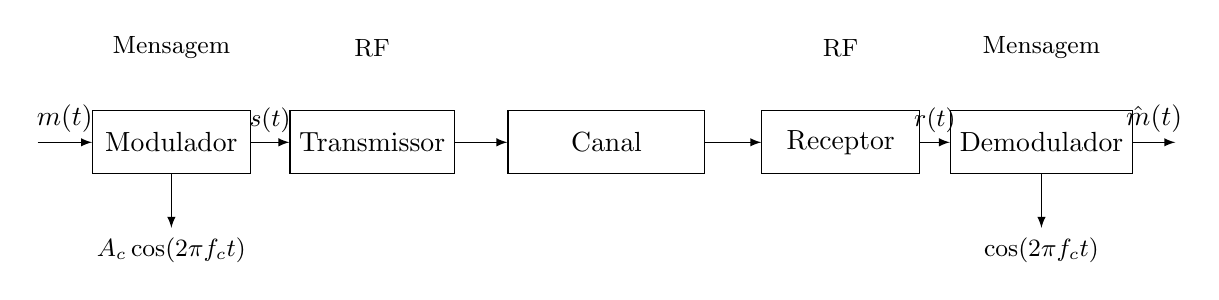
\begin{tikzpicture}[>=latex, scale=0.85]
% Transmissor
\node[draw, rectangle, minimum width=2cm, minimum height=0.8cm] (mod) at (0,0) {Modulador};
\node[draw, rectangle, minimum width=2cm, minimum height=0.8cm] (tx) at (3,0) {Transmissor};

% Canal
\node[draw, rectangle, minimum width=2.5cm, minimum height=0.8cm] (canal) at (6.5,0) {Canal};

% Receptor
\node[draw, rectangle, minimum width=2cm, minimum height=0.8cm] (rx) at (10,0) {Receptor};
\node[draw, rectangle, minimum width=2cm, minimum height=0.8cm] (demod) at (13,0) {Demodulador};

% Conexões
\draw[->] (-2,0) -- node[above] {$m(t)$} (mod.west);
\draw[->] (mod.east) -- node[above, font=\small] {$s(t)$} (tx.west);
\draw[->] (tx.east) -- (canal.west);
\draw[->] (canal.east) -- (rx.west);
\draw[->] (rx.east) -- node[above, font=\small] {$r(t)$} (demod.west);
\draw[->] (demod.east) -- node[above] {$\hat{m}(t)$} (15,0);

% Portadora
\draw[->] (mod.south) -- ++(0,-0.8) node[below, font=\small] {$A_c\cos(2\pi f_c t)$};
\draw[->] (demod.south) -- ++(0,-0.8) node[below, font=\small] {$\cos(2\pi f_c t)$};

% Labels
\node[above of=mod, node distance=1.2cm, font=\small] {Mensagem};
\node[above of=tx, node distance=1.2cm, font=\small] {RF};
\node[above of=rx, node distance=1.2cm, font=\small] {RF};
\node[above of=demod, node distance=1.2cm, font=\small] {Mensagem};
\end{tikzpicture}
\end{center}

\textbf{Componentes principais:}
\begin{itemize}
\item \textbf{Modulador:} Combina mensagem $m(t)$ com portadora
\item \textbf{Canal:} Meio de transmissão (ar, cabo, fibra)
\item \textbf{Demodulador:} Recupera $m(t)$ do sinal modulado
\end{itemize}

\end{frame}

% ============================================

\subsection{AM DSB-SC}

\begin{frame}{AM DSB-SC: Double Sideband Suppressed Carrier}

\begin{block}{Definição}
\textbf{Modulação DSB-SC:}
\[
s(t) = A_c m(t) \cos(2\pi f_c t)
\]
onde:
\begin{itemize}
\item $m(t)$: sinal modulante (mensagem) com largura de banda $W$
\item $A_c$: amplitude da portadora
\item $f_c$: frequência da portadora ($f_c \gg W$)
\end{itemize}
\end{block}

\textbf{Características:}
\begin{itemize}
\item Amplitude varia linearmente com $m(t)$
\item Portadora suprimida (não transmitida)
\item Simples de gerar: multiplicador
\item Requer detecção coerente para demodulação
\end{itemize}

\end{frame}

% ============================================

\begin{frame}{Análise Espectral do DSB-SC}

\textbf{Transformada de Fourier de} $s(t) = A_c m(t) \cos(2\pi f_c t)$:

Usando $\cos(2\pi f_c t) = \frac{e^{j2\pi f_c t} + e^{-j2\pi f_c t}}{2}$:

\[
s(t) = A_c m(t) \frac{e^{j2\pi f_c t} + e^{-j2\pi f_c t}}{2}
\]

Pela propriedade de deslocamento em frequência:
\[
m(t)e^{j2\pi f_c t} \xleftrightarrow{\mathcal{F}} M(f - f_c)
\]

Portanto:
\[
S(f) = \frac{A_c}{2}[M(f - f_c) + M(f + f_c)]
\]

\textbf{Interpretação:}
\begin{itemize}
\item Espectro de $m(t)$ deslocado para $\pm f_c$
\item \textbf{Banda Lateral Superior (USB):} $f_c$ a $f_c + W$
\item \textbf{Banda Lateral Inferior (LSB):} $f_c - W$ a $f_c$
\end{itemize}

\end{frame}

% ============================================

\begin{frame}{Largura de Banda do DSB-SC}

\[
\boxed{S(f) = \frac{A_c}{2}[M(f - f_c) + M(f + f_c)]}
\]

\textbf{Análise da largura de banda:}

\begin{itemize}
\item Mensagem $m(t)$ tem largura de banda $W$ (de $-W$ a $W$)
\item Após modulação:
  \begin{itemize}
  \item USB ocupa: $f_c$ a $f_c + W$
  \item LSB ocupa: $f_c - W$ a $f_c$
  \end{itemize}
\item Largura de banda total do sinal modulado:
\end{itemize}

\[
\boxed{B_{\DSB} = 2W}
\]

\textbf{Observações:}
\begin{itemize}
\item Ambas bandas laterais carregam a mesma informação
\item Redundância espectral
\item Oportunidade para economia de banda $\rightarrow$ SSB
\end{itemize}

\end{frame}

% ============================================

\begin{frame}{Potência do DSB-SC}

\textbf{Potência transmitida:}

\[
P_s = \frac{1}{T} \int_0^T |s(t)|^2 dt = \frac{1}{T} \int_0^T A_c^2 m^2(t) \cos^2(2\pi f_c t) dt
\]

Usando $\langle \cos^2(2\pi f_c t) \rangle = 1/2$:

\[
P_s = \frac{A_c^2}{2} \langle m^2(t) \rangle = \frac{A_c^2}{2} P_m
\]

onde $P_m$ é a potência média de $m(t)$.

\begin{block}{Potência do DSB-SC}
\[
\boxed{P_s = \frac{A_c^2 P_m}{2}}
\]
\end{block}

\textbf{Observação:}
\begin{itemize}
\item Toda potência está nas bandas laterais
\item Nenhuma potência na portadora (suprimida)
\item Eficiência energética superior ao AM convencional
\end{itemize}

\end{frame}

% ============================================

\begin{frame}{Exemplo 1: DSB-SC com Tom Único}

\textbf{Sinal modulante:} $m(t) = \cos(2\pi f_m t)$

\textbf{Sinal DSB-SC:}
\[
s(t) = A_c \cos(2\pi f_m t) \cos(2\pi f_c t)
\]

Usando identidade trigonométrica:
\[
\cos A \cos B = \frac{1}{2}[\cos(A-B) + \cos(A+B)]
\]

\[
s(t) = \frac{A_c}{2}[\cos(2\pi(f_c - f_m)t) + \cos(2\pi(f_c + f_m)t)]
\]

\textbf{Componentes espectrais:}
\begin{itemize}
\item LSB em $f_c - f_m$: amplitude $A_c/2$
\item USB em $f_c + f_m$: amplitude $A_c/2$
\item \textbf{Não há componente em $f_c$!}
\end{itemize}

\textbf{Potência:}
\[
P_s = 2 \times \frac{(A_c/2)^2}{2} = \frac{A_c^2}{4}
\]

\end{frame}

% ============================================

\begin{frame}{Demodulação Coerente do DSB-SC}

\textbf{Detector de Produto (Síncrono):}

\begin{center}
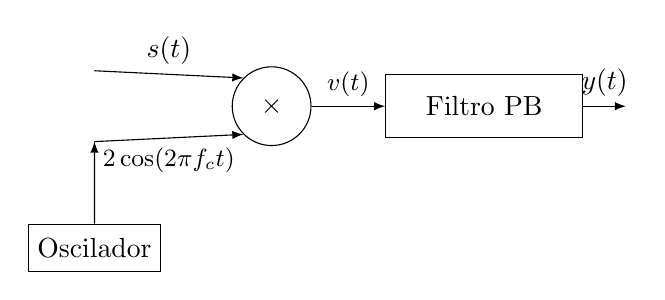
\begin{tikzpicture}[>=latex, scale=0.9]
% Multiplicador
\node[draw, circle, minimum size=1cm] (mult) at (0,0) {$\times$};
% Filtro passa-baixas
\node[draw, rectangle, minimum width=2.5cm, minimum height=0.8cm] (lpf) at (3,0) {Filtro PB};

% Entradas
\draw[->] (-2.5,0.5) -- node[above] {$s(t)$} (mult.north west);
\draw[->] (-2.5,-0.5) -- node[below, font=\small] {$2\cos(2\pi f_c t)$} (mult.south west);

% Saídas
\draw[->] (mult.east) -- node[above, font=\small] {$v(t)$} (lpf.west);
\draw[->] (lpf.east) -- node[above] {$y(t)$} (5,0);

% Oscilador local
\node[draw, rectangle, minimum width=1.5cm, minimum height=0.6cm] (osc) at (-2.5,-2) {Oscilador};
\draw[->] (osc.north) -- (-2.5,-0.5);
\end{tikzpicture}
\end{center}

\textbf{Análise matemática:}

Sinal recebido: $r(t) = A_c m(t) \cos(2\pi f_c t)$

Após multiplicação com $2\cos(2\pi f_c t)$:
\[
v(t) = 2A_c m(t) \cos^2(2\pi f_c t) = A_c m(t) [1 + \cos(4\pi f_c t)]
\]

\[
= A_c m(t) + A_c m(t) \cos(4\pi f_c t)
\]

Após filtro passa-baixas (remove $2f_c$):
\[
\boxed{y(t) = A_c m(t)}
\]

\textbf{Recuperação perfeita com ganho $A_c$!}

\end{frame}

% ============================================

\begin{frame}{Efeito de Erro de Fase na Demodulação}

\textbf{Oscilador local com erro de fase:} $2\cos(2\pi f_c t + \theta)$

Após multiplicação:
\[
v(t) = 2A_c m(t) \cos(2\pi f_c t) \cos(2\pi f_c t + \theta)
\]

Usando $\cos A \cos B = \frac{1}{2}[\cos(A-B) + \cos(A+B)]$:

\[
v(t) = A_c m(t) [\cos\theta + \cos(4\pi f_c t + \theta)]
\]

Após filtro passa-baixas:
\[
\boxed{y(t) = A_c m(t) \cos\theta}
\]

\textbf{Observações:}
\begin{itemize}
\item Atenuação por fator $\cos\theta$
\item Para $\theta = 90^{\circ}$: $y(t) = 0$ (perda total!)
\item Para $\theta pequeno$: $\cos\theta \approx 1$ (pouca degradação)
\item \textbf{Sincronização precisa é crítica!}
\end{itemize}

\end{frame}

% ============================================

\subsection{AM Convencional}

\begin{frame}{AM Convencional (DSB-LC)}

\textbf{Motivação:} DSB-SC requer sincronização perfeita. Podemos simplificar o receptor?

\begin{block}{Definição: AM Convencional}
\[
s(t) = A_c[1 + k_a m(t)] \cos(2\pi f_c t)
\]
onde:
\begin{itemize}
\item $k_a$: sensibilidade ou constante de modulação
\item $1 + k_a m(t)$: envelope do sinal
\item Condição: $|k_a m(t)| \leq 1$ (evitar supermodulação)
\end{itemize}
\end{block}

\textbf{Diferença fundamental:}
\[
s(t) = \underbrace{A_c \cos(2\pi f_c t)}_{\text{portadora}} + \underbrace{A_c k_a m(t) \cos(2\pi f_c t)}_{\text{DSB-SC}}
\]

Portadora transmitida + bandas laterais

\end{frame}

% ============================================

\begin{frame}{Índice de Modulação}

\textbf{Normalização:} Assumir $m(t)$ normalizado tal que $\max|m(t)| = 1$

\textbf{Índice de modulação:}
\[
\mu = k_a \max|m(t)| = k_a
\]

Para $0 \leq \mu \leq 1$:

\[
\boxed{s(t) = A_c[1 + \mu m_n(t)] \cos(2\pi f_c t)}
\]

onde $m_n(t)$ é $m(t)$ normalizado ($\max|m_n(t)| = 1$).

\vspace{0.3cm}

\textbf{Envelope:}
\[
A(t) = A_c[1 + \mu m_n(t)]
\]

\begin{itemize}
\item $\mu = 0$: portadora não modulada
\item $\mu = 1$: modulação 100\% (envelope vai a zero)
\item $\mu > 1$: \textbf{supermodulação} (distorção!)
\end{itemize}

\end{frame}

% ============================================

\begin{frame}{Supermodulação}

\textbf{Condição de supermodulação:} $\mu > 1$ ou $|k_a m(t)| > 1$

\textbf{Problema:}
\[
1 + k_a m(t) < 0 \quad \text{para alguns valores de } t
\]

Envelope torna-se negativo $\rightarrow$ inversão de fase $\rightarrow$ distorção

\vspace{0.5cm}

\textbf{Consequências:}
\begin{itemize}
\item Detector de envelope produz saída distorcida
\item Espectro contém componentes espúrias
\item Ineficiência de potência
\item \textbf{Deve ser evitada!}
\end{itemize}

\vspace{0.3cm}

\textbf{Solução:} Controle automático de ganho (AGC) no transmissor

\textbf{Veja figura:} Comparação de envelopes para $\mu = 0.5$, $1.0$ e $1.5$

\end{frame}

% ============================================

\begin{frame}{Espectro do AM Convencional}

\[
s(t) = A_c \cos(2\pi f_c t) + A_c k_a m(t) \cos(2\pi f_c t)
\]

\textbf{Transformada de Fourier:}
\[
S(f) = \frac{A_c}{2}[\delta(f - f_c) + \delta(f + f_c)] + \frac{A_c k_a}{2}[M(f - f_c) + M(f + f_c)]
\]

\textbf{Componentes:}
\begin{itemize}
\item \textbf{Portadora:} impulsos em $\pm f_c$ com amplitude $A_c/2$
\item \textbf{Bandas laterais:} versões deslocadas de $M(f)$
  \begin{itemize}
  \item USB: $f_c$ a $f_c + W$
  \item LSB: $f_c - W$ a $f_c$
  \end{itemize}
\end{itemize}

\textbf{Largura de banda:}
\[
B_{\AM} = 2W \quad \text{(mesma que DSB-SC)}
\]

\textbf{Diferença visual:} Presença de linhas espectrais em $\pm f_c$

\end{frame}

% ============================================

\begin{frame}{Potência do AM Convencional}

\[
s(t) = A_c[1 + k_a m(t)] \cos(2\pi f_c t)
\]

\textbf{Potência total:}
\[
P_s = \left\langle A_c^2[1 + k_a m(t)]^2 \cos^2(2\pi f_c t) \right\rangle
\]

\[
= \frac{A_c^2}{2} \left\langle [1 + k_a m(t)]^2 \right\rangle
\]

\[
= \frac{A_c^2}{2} \left[1 + 2k_a\langle m(t)\rangle + k_a^2\langle m^2(t)\rangle\right]
\]

Se $\langle m(t)\rangle = 0$ (sem componente DC):

\[
P_s = \frac{A_c^2}{2}[1 + k_a^2 P_m]
\]

\textbf{Decomposição:}
\begin{itemize}
\item Potência na portadora: $P_c = \frac{A_c^2}{2}$
\item Potência nas bandas laterais: $P_{sb} = \frac{A_c^2 k_a^2 P_m}{2}$
\end{itemize}

\end{frame}

% ============================================

\begin{frame}{Eficiência de Potência do AM}

\textbf{Eficiência:} Fração da potência total que carrega informação

\[
\eta = \frac{P_{sb}}{P_s} = \frac{P_{sb}}{P_c + P_{sb}}
\]

\[
= \frac{\frac{A_c^2 k_a^2 P_m}{2}}{\frac{A_c^2}{2} + \frac{A_c^2 k_a^2 P_m}{2}} = \frac{k_a^2 P_m}{1 + k_a^2 P_m}
\]

\textbf{Para tom único} $m(t) = \cos(2\pi f_m t)$: $P_m = 1/2$

\[
\eta = \frac{\mu^2/2}{1 + \mu^2/2} = \frac{\mu^2}{2 + \mu^2}
\]

\textbf{Eficiências típicas:}
\begin{itemize}
\item $\mu = 0.5$: $\eta = 11\%$
\item $\mu = 1.0$: $\eta = 33\%$ (máximo!)
\item $\mu = 0.3$: $\eta = 4.3\%$
\end{itemize}

\textbf{Conclusão:} AM convencional é \textbf{muito ineficiente} em potência!

\end{frame}

% ============================================

\begin{frame}{Exemplo 2: AM Convencional com Tom Único}

\textbf{Dado:} $m(t) = \cos(2\pi f_m t)$, $\mu = 0.8$, $A_c = 100$ V

\textbf{Sinal AM:}
\[
s(t) = 100[1 + 0.8\cos(2\pi f_m t)] \cos(2\pi f_c t)
\]

\textbf{Espectro:}
\begin{itemize}
\item Portadora em $f_c$: amplitude $50$ V
\item LSB em $f_c - f_m$: amplitude $40 \times 0.5 = 20$ V
\item USB em $f_c + f_m$: amplitude $20$ V
\end{itemize}

\textbf{Potências:}
\[
P_c = \frac{100^2}{2} = 5000 \text{ W (em 1 }\Omega\text{)}
\]
\[
P_{sb} = \frac{0.8^2}{2} \times 5000 = 1600 \text{ W}
\]
\[
P_s = 5000 + 1600 = 6600 \text{ W}
\]
\[
\eta = \frac{1600}{6600} = 24.2\%
\]

\end{frame}

% ============================================

\begin{frame}{Detector de Envelope}

\textbf{Vantagem do AM convencional:} Demodulação simples com detector de envelope

\begin{center}
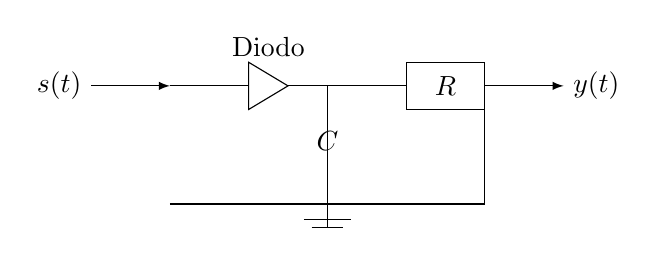
\begin{tikzpicture}[>=latex, scale=1.0]
% Diodo
\draw (0,0) -- (1,0);
\draw[fill=white] (1,-0.3) -- (1,0.3) -- (1.5,0) -- cycle;
\draw (1.5,0) -- (2,0);
% Capacitor
\draw (2,0) -- (2,-1.5);
\draw (1.7,-1.5) -- (2.3,-1.5);
\draw (1.7,-1.7) -- (2.3,-1.7);
% Resistor
\draw (2,0) -- (3,0);
\draw (3,-0.3) rectangle (4,0.3);
\node at (3.5,0) {$R$};
\draw (4,0) -- (4,-1.5);
% Terra
\draw (0,-1.5) -- (4,-1.5);
\draw (2,-1.8) -- (2,-1.5);
\draw (1.8,-1.8) -- (2.2,-1.8);
% Entrada/Saída
\draw[<-] (0,0) -- (-1,0) node[left] {$s(t)$};
\draw[->] (4,0) -- (5,0) node[right] {$y(t)$};
% Labels
\node at (2,-0.7) {$C$};
\node at (1.25,0.5) {Diodo};
\end{tikzpicture}
\end{center}

\textbf{Funcionamento:}
\begin{itemize}
\item Diodo retifica o sinal (permite apenas semi-ciclos positivos)
\item Capacitor $C$ carrega rapidamente nos picos
\item Descarrega lentamente através de $R$
\item Saída segue o envelope $A_c[1 + k_a m(t)]$
\end{itemize}

\textbf{Condição para operação correta:}
\[
\frac{1}{f_c} \ll RC \ll \frac{1}{W}
\]

\textbf{Muito mais simples que detecção coerente!} (Razão do sucesso do AM broadcast)

\end{frame}

% ============================================

\subsection{AM SSB}

\begin{frame}{AM SSB: Single Sideband}

\textbf{Observação fundamental:}

No DSB-SC, ambas bandas laterais (USB e LSB) carregam a mesma informação.

\vspace{0.3cm}

\textbf{Ideia do SSB:}

Transmitir apenas uma banda lateral $\rightarrow$ economiza largura de banda!

\vspace{0.5cm}

\textbf{Vantagens do SSB:}
\begin{itemize}
\item Largura de banda: $B_{\SSB} = W$ (metade do DSB!)
\item Potência concentrada em uma banda
\item Menos interferência
\item Melhor para canais seletivos em frequência
\end{itemize}

\textbf{Desvantagens:}
\begin{itemize}
\item Geração mais complexa
\item Demodulação coerente necessária
\item Sensível a erro de frequência
\end{itemize}

\end{frame}

% ============================================

\begin{frame}{Representação Matemática do SSB}

\textbf{SSB pode ser gerado de duas formas:}

1. Filtragem de DSB-SC
2. Método de Hilbert (phasing)

\vspace{0.5cm}

\textbf{Representação usando Transformada de Hilbert:}

\begin{block}{SSB-USB (Upper Sideband)}
\[
s_{\USB}(t) = \frac{A_c}{2}[m(t)\cos(2\pi f_c t) - \hilbert{m}(t)\sin(2\pi f_c t)]
\]
\end{block}

\begin{block}{SSB-LSB (Lower Sideband)}
\[
s_{\LSB}(t) = \frac{A_c}{2}[m(t)\cos(2\pi f_c t) + \hilbert{m}(t)\sin(2\pi f_c t)]
\]
\end{block}

onde $\hilbert{m}(t)$ é a \textbf{transformada de Hilbert} de $m(t)$.

\end{frame}

% ============================================

\begin{frame}{Transformada de Hilbert}

\begin{block}{Definição no Tempo}
\[
\hilbert{m}(t) = m(t) * \frac{1}{\pi t} = \frac{1}{\pi} \int_{-\infty}^{\infty} \frac{m(\tau)}{t - \tau} d\tau
\]
\end{block}

\begin{block}{Definição na Frequência}
\[
\hat{M}(f) = -j\sgn(f) M(f) = \begin{cases}
-jM(f) & f > 0 \\
+jM(f) & f < 0
\end{cases}
\]
\end{block}

\textbf{Interpretação:}
\begin{itemize}
\item Defasador de $-90^{\circ}$ para todas as frequências
\item Para $f > 0$: fase reduzida em $90^{\circ}$
\item Para $f < 0$: fase aumentada em $90^{\circ}$
\end{itemize}

\textbf{Exemplos:}
\begin{itemize}
\item $\hilbert{\cos(2\pi ft)} = \sin(2\pi ft)$
\item $\hilbert{\sin(2\pi ft)} = -\cos(2\pi ft)$
\end{itemize}

\end{frame}

% ============================================

\begin{frame}{Derivação do SSB-USB}

\textbf{Partindo do DSB-SC:} $s_{\DSB}(t) = A_c m(t) \cos(2\pi f_c t)$

Espectro: $S_{\DSB}(f) = \frac{A_c}{2}[M(f - f_c) + M(f + f_c)]$

\vspace{0.3cm}

\textbf{Para obter USB:} Aplicar filtro passa-altas ideal centrado em $f_c$

\[
H_{\USB}(f) = \begin{cases}
1 & f > f_c \\
0 & f < f_c
\end{cases}
\]

No tempo (método de Hilbert):

$m(t)\cos(2\pi f_c t)$ contribui para USB e LSB

$\hilbert{m}(t)\sin(2\pi f_c t)$ contribui para USB e LSB com fases opostas

\vspace{0.3cm}

\textbf{Combinação que cancela LSB:}
\[
s_{\USB}(t) = \frac{A_c}{2}[m(t)\cos(2\pi f_c t) - \hilbert{m}(t)\sin(2\pi f_c t)]
\]

LSB se cancela, USB permanece!

\end{frame}

% ============================================

\begin{frame}{Espectro do SSB}

\textbf{SSB-USB:}
\[
S_{\USB}(f) = \begin{cases}
\frac{A_c}{2}M(f - f_c) & f > 0 \\
\frac{A_c}{2}M(f + f_c) & f < 0
\end{cases}
\]

Apenas banda superior em torno de $f_c$!

\vspace{0.5cm}

\textbf{Largura de banda:}
\[
\boxed{B_{\SSB} = W}
\]

\textbf{Economia de 50\% comparado a DSB!}

\vspace{0.5cm}

\textbf{Potência:}
\[
P_{\SSB} = \frac{A_c^2 P_m}{4}
\]

Metade da potência do DSB-SC (uma banda lateral em vez de duas).

\end{frame}

% ============================================

\begin{frame}{Geração de SSB: Método do Filtro}

\begin{center}
\begin{tikzpicture}[>=latex, scale=0.85]
% Multiplicador
\node[draw, circle, minimum size=0.8cm] (mult) at (0,0) {$\times$};
% Filtro
\node[draw, rectangle, minimum width=2.2cm, minimum height=0.7cm] (filt) at (3,0) {Filtro SSB};
% Amplificador
\node[draw, rectangle, minimum width=1.5cm, minimum height=0.7cm] (amp) at (6,0) {Amp.};

% Conexões
\draw[->] (-2,0.4) -- node[above, font=\small] {$m(t)$} (mult.north west);
\draw[->] (-2,-0.4) -- node[below, font=\small] {$A_c\cos(2\pi f_c t)$} (mult.south west);
\draw[->] (mult.east) -- node[above, font=\small] {DSB-SC} (filt.west);
\draw[->] (filt.east) -- (amp.west);
\draw[->] (amp.east) -- node[above, font=\small] {$s_{\SSB}(t)$} (7.5,0);

% Resposta do filtro
\node[below of=filt, node distance=1.8cm, font=\footnotesize] (resp) {
\begin{tikzpicture}[scale=0.4]
\draw[->] (-2,0) -- (2,0) node[right] {$f$};
\draw[->] (0,-0.3) -- (0,1.5) node[above] {$|H|$};
\draw[thick, blue] (-2,0) -- (-0.3,0) -- (-0.1,1.2) -- (2,1.2);
\node[below] at (-0.2,-0.3) {$f_c$};
\end{tikzpicture}
};
\end{tikzpicture}
\end{center}

\textbf{Processo:}
\begin{enumerate}
\item Gerar DSB-SC: $A_c m(t)\cos(2\pi f_c t)$
\item Filtrar com passa-faixas centrado em $f_c$
   \begin{itemize}
   \item USB: passa alta de $f_c$
   \item LSB: passa baixa de $f_c$
   \end{itemize}
\item Amplificar
\end{enumerate}

\textbf{Desafio:} Filtro deve ter transição abrupta em $f_c$ (difícil para sinais com componentes de baixa frequência)

\end{frame}

% ============================================

\begin{frame}{Geração de SSB: Método de Hilbert}

\begin{center}
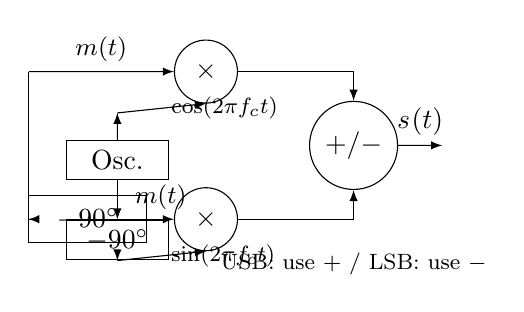
\begin{tikzpicture}[>=latex, scale=0.75]
% Branch superior
\node[draw, circle, minimum size=0.8cm] (mult1) at (2,1.5) {$\times$};
\draw[->] (-1,1.5) -- node[above, font=\small] {$m(t)$} (mult1.west);
\draw[->] (0.5,0.8) -- node[right, font=\footnotesize] {$\cos(2\pi f_c t)$} (mult1.south);

% Branch inferior
\node[draw, rectangle, minimum width=1.5cm, minimum height=0.6cm] (hilb) at (0,-1) {$-90^{\circ}$};
\node[draw, circle, minimum size=0.8cm] (mult2) at (2,-1) {$\times$};
\draw[->] (-1,1.5) |- (hilb.west);
\draw[->] (hilb.east) -- node[above, font=\small] {$\hilbert{m}(t)$} (mult2.west);
\draw[->] (0.5,-1.7) -- node[right, font=\footnotesize] {$\sin(2\pi f_c t)$} (mult2.south);

% Somador
\node[draw, circle, minimum size=0.8cm] (sum) at (4.5,0.25) {$+/-$};
\draw[->] (mult1.east) -| (sum.north);
\draw[->] (mult2.east) -| (sum.south);
\draw[->] (sum.east) -- node[above] {$s_{\SSB}(t)$} (6,0.25);

% Oscilador em fase
\node[draw, rectangle, minimum width=1.3cm, minimum height=0.5cm] (osc) at (0.5,0) {Osc.};
\draw[->] (osc.north) -- (0.5,0.8);
\node[draw, rectangle, minimum width=1.3cm, minimum height=0.5cm] (def) at (0.5,-1.35) {$-90^{\circ}$};
\draw[->] (osc.south) -- (def.north);
\draw[->] (def.south) -- (0.5,-1.7);

% Labels
\node[below of=sum, node distance=1.5cm, font=\footnotesize] {USB: use $+$ / LSB: use $-$};
\end{tikzpicture}
\end{center}

\textbf{Características:}
\begin{itemize}
\item Não requer filtros seletivos
\item Defasador de $-90^{\circ}$ (implementado com all-pass networks)
\item Dois osciladores em quadratura (defasados $90^{\circ}$)
\item Escolha do sinal no somador determina USB ou LSB
\end{itemize}

\textbf{Desafio:} Casamento preciso de amplitude e fase nos dois ramos

\end{frame}

% ============================================

\begin{frame}{Demodulação do SSB}

\textbf{SSB requer detecção coerente:}

\begin{center}
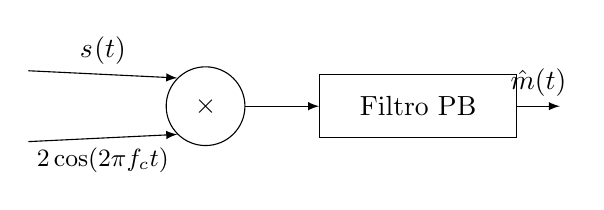
\begin{tikzpicture}[>=latex, scale=0.9]
\node[draw, circle, minimum size=1cm] (mult) at (0,0) {$\times$};
\node[draw, rectangle, minimum width=2.5cm, minimum height=0.8cm] (lpf) at (3,0) {Filtro PB};
\draw[->] (-2.5,0.5) -- node[above] {$s_{\SSB}(t)$} (mult.north west);
\draw[->] (-2.5,-0.5) -- node[below, font=\small] {$2\cos(2\pi f_c t)$} (mult.south west);
\draw[->] (mult.east) -- (lpf.west);
\draw[->] (lpf.east) -- node[above] {$\hat{m}(t)$} (5,0);
\end{tikzpicture}
\end{center}

\textbf{Sensibilidade a erro de frequência:}

Se oscilador local tem erro $\Delta f$:
\[
\hat{m}(t) = m(t) \cos(2\pi\Delta f \cdot t)
\]

Sinal recuperado tem modulação residual em $\Delta f$!

\vspace{0.3cm}

\textbf{Para voz:} $\Delta f < 20$ Hz é aceitável

\textbf{Para música:} $\Delta f < 2$ Hz necessário

\textbf{Solução:} Transmitir piloto de baixa potência para sincronização

\end{frame}

% ============================================

\begin{frame}{Exemplo 3: Comparação DSB vs SSB}

\textbf{Sinal modulante:} $m(t)$ com largura de banda $W = 5$ kHz

\textbf{Frequência da portadora:} $f_c = 1$ MHz

\vspace{0.5cm}

\textbf{Comparação:}

\begin{center}
\begin{tabular}{|l|c|c|}
\hline
\textbf{Característica} & \textbf{DSB-SC} & \textbf{SSB} \\
\hline
Largura de banda & $2W = 10$ kHz & $W = 5$ kHz \\
\hline
Potência (relativa) & $1.0$ & $0.5$ \\
\hline
Geração & Simples & Complexa \\
\hline
Demodulação & Coerente & Coerente \\
\hline
Sensibilidade $\Delta f$ & Baixa & Alta \\
\hline
Aplicações & Estéreo FM & Rádio amador \\
& & Comunicação longa distância \\
\hline
\end{tabular}
\end{center}

\textbf{Trade-off:} Economia de banda vs. complexidade

\end{frame}

% ============================================

\subsection{AM VSB}

\begin{frame}{AM VSB: Vestigial Sideband}

\textbf{Problema com SSB:}

Filtragem abrupta em $f_c$ é difícil, especialmente para sinais com componentes DC ou de muito baixa frequência (ex: vídeo).

\vspace{0.3cm}

\textbf{Solução: VSB}

Transmitir uma banda lateral completa + "vestígio" da outra.

\begin{block}{Definição}
VSB é um compromisso entre DSB e SSB:
\begin{itemize}
\item Largura de banda: $W < B_{\VSB} < 2W$
\item Transmite USB completa + parte da LSB (ou vice-versa)
\item Filtro com roll-off gradual em $f_c$
\end{itemize}
\end{block}

\textbf{Aplicação principal:} TV analógica (NTSC, PAL)

Vídeo tem componentes de 0 Hz a vários MHz $\rightarrow$ SSB impraticável

\end{frame}

% ============================================

\begin{frame}{Filtro VSB}

\textbf{Característica do filtro VSB:}

\begin{center}
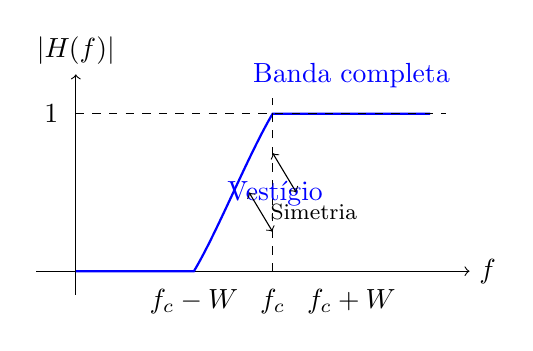
\begin{tikzpicture}[scale=1.0]
\draw[->] (-0.5,0) -- (5,0) node[right] {$f$};
\draw[->] (0,-0.3) -- (0,2.5) node[above] {$|H_{\VSB}(f)|$};

% Filtro VSB
\draw[thick, blue] (0,0) -- (1.5,0) 
    .. controls (1.8,0.5) and (2.2,1.5) .. 
    (2.5,2) -- (4.5,2);

% Linhas de referência
\draw[dashed] (2.5,0) -- (2.5,2.2);
\draw[dashed] (0,2) -- (4.7,2);

% Labels
\node[below] at (2.5,-0.1) {$f_c$};
\node[left] at (-0.1,2) {$1$};
\node[below] at (1.5,-0.1) {$f_c-W$};
\node[below] at (3.5,-0.1) {$f_c+W$};
\node[above right, blue] at (1.8,0.7) {Vestígio};
\node[above, blue] at (3.5,2.2) {Banda completa};

% Simetria vestigial
\draw[<->] (2.5,0.5) -- (2.2,1) node[midway, right, font=\footnotesize] {Simetria};
\draw[<->] (2.5,1.5) -- (2.8,1);
\end{tikzpicture}
\end{center}

\textbf{Condição de simetria vestigial:}
\[
H_{\VSB}(f_c + f) + H_{\VSB}(f_c - f) = \text{constante}
\]

Garante recuperação sem distorção na demodulação coerente.

\end{frame}

% ============================================

\begin{frame}{Análise Matemática do VSB}

\textbf{Sinal VSB:}
\[
s_{\VSB}(t) = [A_c m(t) \cos(2\pi f_c t)] * h_{\VSB}(t)
\]

\textbf{No domínio da frequência:}
\[
S_{\VSB}(f) = \frac{A_c}{2}[M(f - f_c) + M(f + f_c)] H_{\VSB}(f)
\]

\textbf{Demodulação coerente com} $2\cos(2\pi f_c t)$:

Produto resulta em:
\[
v(t) = s_{\VSB}(t) \cdot 2\cos(2\pi f_c t)
\]

Após passa-baixas, se $H_{\VSB}$ satisfaz condição de simetria:
\[
\boxed{y(t) = A_c m(t)}
\]

\textbf{Recuperação perfeita!}

\end{frame}

% ============================================

\begin{frame}{VSB na TV Analógica}

\textbf{Sistema NTSC (EUA):}

\begin{itemize}
\item Sinal de vídeo: 0 a 4.2 MHz
\item Frequência de portadora visual: $f_v$
\item Largura do canal: 6 MHz total
\end{itemize}

\textbf{Alocação espectral:}
\begin{itemize}
\item Vestígio LSB: 1.25 MHz abaixo de $f_v$
\item USB completa: 4.2 MHz acima de $f_v$
\item Portadora de áudio FM: 4.5 MHz acima de $f_v$
\end{itemize}

\textbf{Economia de banda:}
\begin{itemize}
\item DSB precisaria: $2 \times 4.2 = 8.4$ MHz
\item VSB usa: $1.25 + 4.2 = 5.45$ MHz
\item Economia: $\approx 35\%$
\end{itemize}

\textbf{Trade-off perfeito:} Eficiência espectral + facilidade de implementação

\end{frame}

% ============================================

\begin{frame}{Largura de Banda do VSB}

\textbf{Largura de banda geral:}
\[
B_{\VSB} = W + f_{vest}
\]

onde $f_{vest}$ é a largura do vestígio.

\vspace{0.3cm}

\textbf{Limites:}
\begin{itemize}
\item Se $f_{vest} = W$: $B_{\VSB} = 2W$ (torna-se DSB)
\item Se $f_{vest} = 0$: $B_{\VSB} = W$ (torna-se SSB)
\end{itemize}

\textbf{Típico:} $f_{vest} = 0.2W$ a $0.3W$

\[
\boxed{W < B_{\VSB} < 2W}
\]

\textbf{Exemplo NTSC:}
\begin{itemize}
\item $W = 4.2$ MHz
\item $f_{vest} = 1.25$ MHz
\item $B_{\VSB} = 5.45$ MHz $\approx 1.3W$
\end{itemize}

\end{frame}

% ============================================

\subsection{Comparação}

\begin{frame}{Tabela Comparativa: Tipos de AM}

\begin{center}
\footnotesize
\begin{tabular}{|l|c|c|c|c|}
\hline
\textbf{Tipo} & \textbf{DSB-SC} & \textbf{AM Conv.} & \textbf{SSB} & \textbf{VSB} \\
\hline
Largura de banda & $2W$ & $2W$ & $W$ & $W<B<2W$ \\
\hline
Potência (relativa) & $1.0$ & $>3.0$ & $0.5$ & $\approx 0.7$ \\
\hline
Eficiência potência & Alta & Baixa & Máxima & Alta \\
& & $(< 33\%)$ & & \\
\hline
Geração & Simples & Simples & Complexa & Moderada \\
\hline
Demodulação & Coerente & Envelope & Coerente & Coerente \\
\hline
Complexidade RX & Média & Mínima & Alta & Média \\
\hline
Sensibilidade $\Delta f$ & Baixa & N/A & Alta & Média \\
\hline
Aplicações & - & Rádio AM & Rádio & TV \\
& & broadcast & amador & analógica \\
\hline
\end{tabular}
\end{center}

\vspace{0.3cm}

\textbf{Escolha depende de:}
\begin{itemize}
\item Largura de banda disponível
\item Potência disponível
\item Complexidade aceitável no TX e RX
\item Custo
\end{itemize}

\end{frame}

% ============================================

\begin{frame}{Comparação Espectral Visual}

\textbf{Para mesmo sinal modulante} $m(t)$ com banda $W$:

\begin{center}
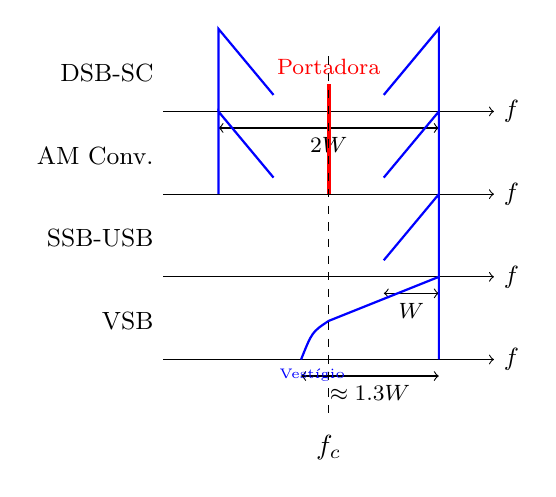
\begin{tikzpicture}[scale=0.7]
% DSB-SC
\begin{scope}[yshift=3cm]
\draw[->] (-3,0) -- (3,0) node[right, font=\small] {$f$};
\draw[thick, blue] (-2,0) -- (-2,1.5) -- (-1,0.3);
\draw[thick, blue] (1,0.3) -- (2,1.5) -- (2,0);
\node[left, font=\small] at (-3,0.7) {DSB-SC};
\draw[<->] (-2,-0.3) -- (2,-0.3) node[midway, below, font=\footnotesize] {$2W$};
\end{scope}

% AM Convencional
\begin{scope}[yshift=1.5cm]
\draw[->] (-3,0) -- (3,0) node[right, font=\small] {$f$};
\draw[thick, blue] (-2,0) -- (-2,1.5) -- (-1,0.3);
\draw[thick, blue] (1,0.3) -- (2,1.5) -- (2,0);
\draw[thick, red, line width=1.5pt] (0,0) -- (0,2);
\node[left, font=\small] at (-3,0.7) {AM Conv.};
\node[above, red, font=\footnotesize] at (0,2) {Portadora};
\end{scope}

% SSB
\begin{scope}[yshift=0cm]
\draw[->] (-3,0) -- (3,0) node[right, font=\small] {$f$};
\draw[thick, blue] (1,0.3) -- (2,1.5) -- (2,0);
\node[left, font=\small] at (-3,0.7) {SSB-USB};
\draw[<->] (1,-0.3) -- (2,-0.3) node[midway, below, font=\footnotesize] {$W$};
\end{scope}

% VSB
\begin{scope}[yshift=-1.5cm]
\draw[->] (-3,0) -- (3,0) node[right, font=\small] {$f$};
\draw[thick, blue] (-0.5,0) .. controls (-0.3,0.5) .. (0,0.7) 
                   -- (2,1.5) -- (2,0);
\node[left, font=\small] at (-3,0.7) {VSB};
\draw[<->] (-0.5,-0.3) -- (2,-0.3) node[midway, below, font=\footnotesize] {$\approx 1.3W$};
\node[below, blue, font=\tiny] at (-0.3,0) {Vestígio};
\end{scope}

% fc marca
\draw[dashed] (0,4) -- (0,-2.5);
\node[below] at (0,-2.7) {$f_c$};
\end{tikzpicture}
\end{center}

\end{frame}

% ============================================

\begin{frame}{Aplicações Práticas das Variantes AM}

\textbf{AM Convencional (DSB-LC):}
\begin{itemize}
\item Rádio AM broadcast (535-1705 kHz)
\item Receptor muito simples e barato
\item Ainda usado em países em desenvolvimento
\end{itemize}

\textbf{SSB:}
\begin{itemize}
\item Rádio amador (HF: 3-30 MHz)
\item Comunicações marítimas e aeronáuticas
\item Comunicações militares de longa distância
\item Telefonia por satélite (histórico)
\end{itemize}

\textbf{VSB:}
\begin{itemize}
\item TV analógica terrestre (NTSC, PAL, SECAM)
\item Modems de alta velocidade (histórico)
\item Base para VSB digital (ATSC)
\end{itemize}

\textbf{DSB-SC:}
\begin{itemize}
\item Estéreo em FM (sinal L-R)
\item Componente de cor em TV (QAM)
\end{itemize}

\end{frame}

% ============================================

\begin{frame}{Resumo: Modulação em Amplitude}

\textbf{Conceitos fundamentais:}
\begin{itemize}
\item Modulação desloca espectro de banda base para RF
\item Facilita multiplexação, propagação e processamento
\end{itemize}

\vspace{0.3cm}

\textbf{Quatro variantes principais:}

\begin{enumerate}
\item \textbf{DSB-SC:} $s(t) = A_c m(t)\cos(2\pi f_c t)$
   \begin{itemize}
   \item Simples, mas requer detecção coerente
   \end{itemize}

\item \textbf{AM Convencional:} $s(t) = A_c[1 + k_a m(t)]\cos(2\pi f_c t)$
   \begin{itemize}
   \item Detector de envelope, mas ineficiente ($\eta \leq 33\%$)
   \end{itemize}

\item \textbf{SSB:} Usa transformada de Hilbert
   \begin{itemize}
   \item Economiza largura de banda (50\%)
   \end{itemize}

\item \textbf{VSB:} Compromisso DSB-SSB
   \begin{itemize}
   \item Ideal para sinais com componentes DC/baixa frequência
   \end{itemize}
\end{enumerate}

\textbf{Escolha baseada em:} Banda disponível, potência, complexidade, custo

\end{frame}
